\subsection{Functional coherence audit: g:Profiler finds no pathway signal in predicted or CLIP target sets (negative)}
If the CNN ranks real targets, its top-ranked genes for a miRNA might share biology. We tested this with the g:Profiler g:GOSt service (version \texttt{e114\_eg62\_p19\_27110d83}; \texttt{scripts/gprofiler\_enrichment.py}; \texttt{results/gprofiler\_enrichment.json}; hermetic tests) on 13 well-studied miRNAs. For each miRNA the background is the set of genes scored for that miRNA, and we query four gene sets of size $K=200$: CNN top-$K$, CLIP-positive genes ranked by CNN score, the top-$K$ genes by HEK293 abundance (confound control) and 3 seeded random draws. Terms are called significant under g:SCS, which corrects the one-sided hypergeometric tail
\begin{equation}p=\sum_{i\ge k}\frac{\binom{K_t}{i}\binom{N-K_t}{n-i}}{\binom{N}{n}}\end{equation}
(query size $n$, background $N$, term size $K_t$, overlap $k$) for the dependence among GO terms. Gates, fixed before any group comparison, all passed: a 20-gene canonical cell-cycle positive control recovers GO:0007049 (top hit KEGG cell cycle, $p=3.5\times10^{-31}$); the median random set has 0 significant terms; the median unmapped fraction is 6.75\%.
All three hypotheses are falsified. CNN top-$K$ sets have zero significant terms for 13/13 miRNAs and CLIP-positive sets for 12/13, so neither beats random (H1: 0 wins, 0 losses, $p=1.000$; H2 term overlap with the CLIP set: 0 wins, 0 losses). The expression control returns 47--115 terms per miRNA and beats the CNN on 13/13 (H3, Figure~\ref{fig:gprofiler}).
A post-hoc arm that we did not pre-register swaps to the default whole-genome background: CNN top-$K$ still loses to the first random set (0 wins, 6 losses; median 0 vs 1 terms), consistent with (but not a test of) the CLIP-scored universe being biased toward expressed, well-annotated genes. The reading matches the expression-confound section: at $K=200$, target lists from sequence or CLIP carry no detectable pathway coherence, while abundance alone carries a lot. Pathway enrichment of predicted miRNA targets should not be read as evidence of targeting unless it beats an expression-matched control.
\begin{figure}[h]\centering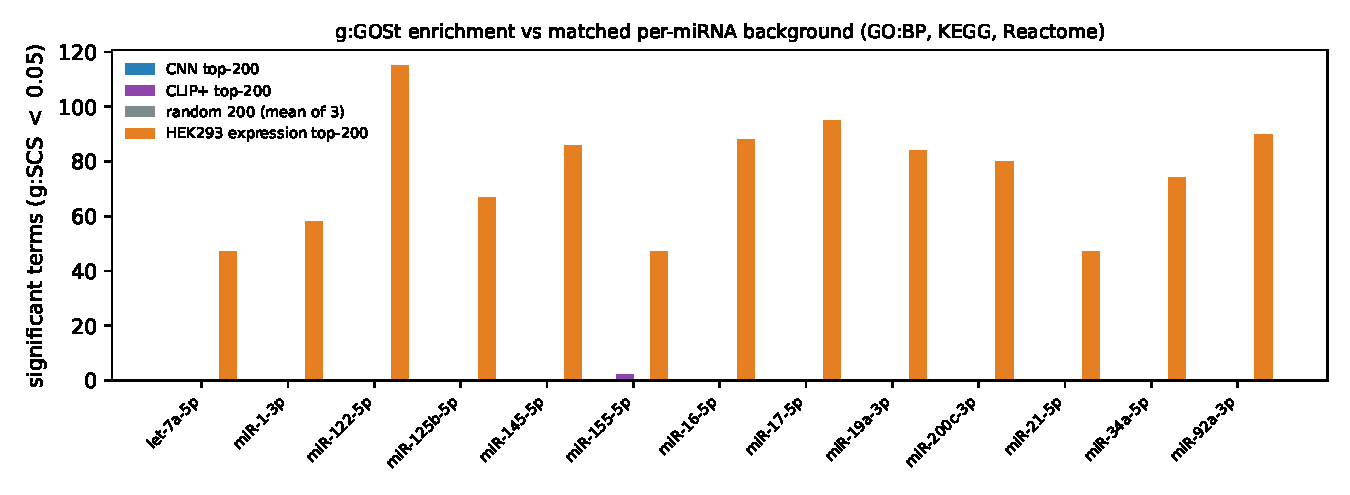
\includegraphics[width=0.95\linewidth]{figs/fig_gprofiler.pdf}
\caption{Significant g:GOSt terms per miRNA for four gene sets of 200 against each miRNA's scored-gene background. Expression top-200 (orange) is the confound control.}\label{fig:gprofiler}\end{figure}
